% generated by Plantuml 1.2024.0       
\definecolor{plantucolor0000}{RGB}{0,0,0}
\definecolor{plantucolor0001}{RGB}{241,241,241}
\definecolor{plantucolor0002}{RGB}{24,24,24}
\definecolor{plantucolor0003}{RGB}{180,167,229}
\definecolor{plantucolor0004}{RGB}{173,209,178}
\definecolor{plantucolor0005}{RGB}{200,41,48}
\definecolor{plantucolor0006}{RGB}{132,190,132}
\definecolor{plantucolor0007}{RGB}{3,128,72}
\definecolor{plantucolor0008}{RGB}{254,255,221}
\definecolor{plantucolor0009}{RGB}{235,147,127}
\scalebox{0.6}{
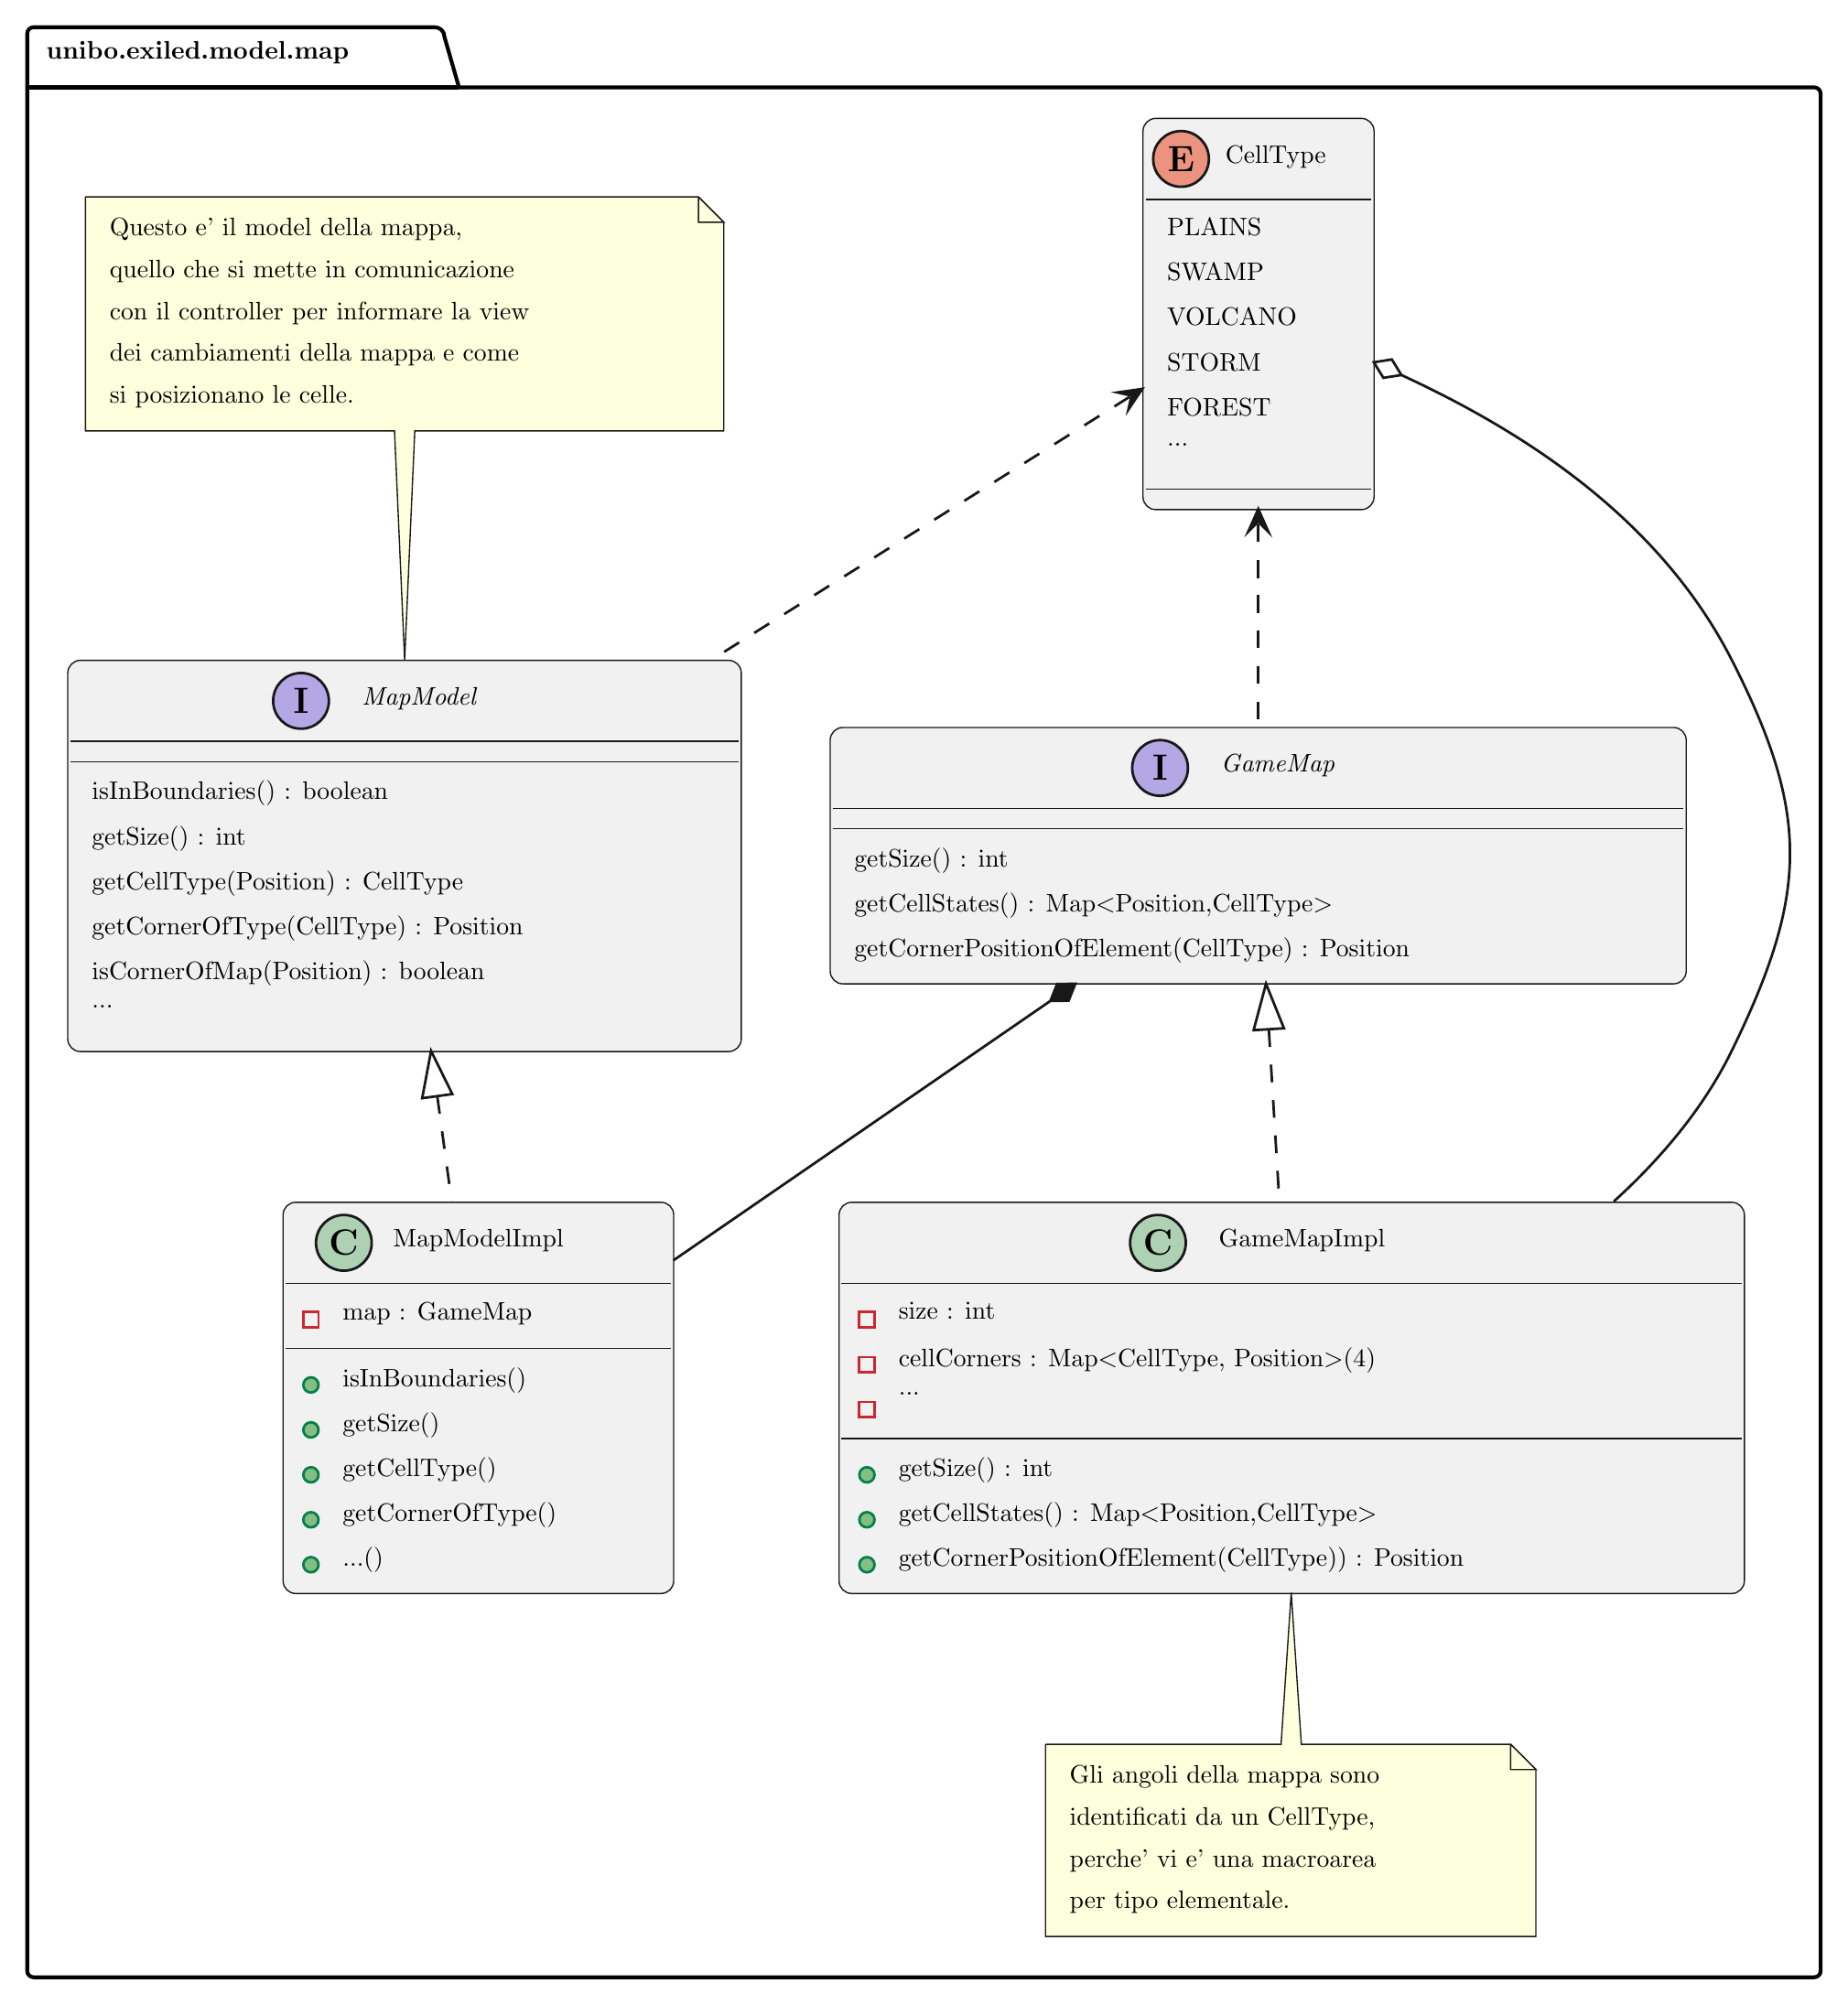
\begin{tikzpicture}[yscale=-1
,pstyle0/.style={color=black,line width=1.5pt}
,pstyle1/.style={color=plantucolor0002,fill=plantucolor0001,line width=0.5pt}
,pstyle2/.style={color=plantucolor0002,fill=plantucolor0003,line width=1.0pt}
,pstyle3/.style={color=plantucolor0002,line width=0.5pt}
,pstyle4/.style={color=plantucolor0002,fill=plantucolor0004,line width=1.0pt}
,pstyle5/.style={color=plantucolor0005,line width=1.0pt}
,pstyle6/.style={color=plantucolor0007,fill=plantucolor0006,line width=1.0pt}
,pstyle7/.style={color=plantucolor0002,fill=plantucolor0008,line width=0.5pt}
,pstyle9/.style={color=plantucolor0002,line width=1.0pt,dash pattern=on 7.0pt off 7.0pt}
,pstyle10/.style={color=plantucolor0002,line width=1.0pt}
,pstyle11/.style={color=plantucolor0002,fill=plantucolor0002,line width=1.0pt}
]
\draw[pstyle0] (8.5pt,6pt) -- (166.9483pt,6pt) arc(270:360:3.75pt)  -- (176.4483pt,29.7461pt) -- (711.5pt,29.7461pt) arc(270:360:2.5pt)  -- (714pt,773.5pt) arc(0:90:2.5pt)  -- (8.5pt,776pt) arc(90:180:2.5pt)  -- (6pt,8.5pt) arc(180:270:2.5pt) ;
\draw[pstyle0] (6pt,29.7461pt) -- (176.4483pt,29.7461pt);
\node at (10pt,8pt)[below right,color=black]{\textbf{unibo.exiled.model.map}};
\draw[pstyle1] (323pt,287.5pt) arc (180:270:5pt) -- (328pt,282.5pt) -- (655.9307pt,282.5pt) arc (270:360:5pt) -- (660.9307pt,287.5pt) -- (660.9307pt,378.7383pt) arc (0:90:5pt) -- (655.9307pt,383.7383pt) -- (328pt,383.7383pt) arc (90:180:5pt) -- (323pt,378.7383pt) -- cycle;
\draw[pstyle2] (453.2306pt,298.5pt) ellipse (11pt and 11pt);
\node at (453.2306pt,298.5pt)[]{\textbf{\Large I}};
\node at (473.7306pt,289.627pt)[below right,color=black]{\textit{GameMap}};
\draw[pstyle3] (324pt,314.5pt) -- (659.9307pt,314.5pt);
\draw[pstyle3] (324pt,322.5pt) -- (659.9307pt,322.5pt);
\node at (329pt,326.5pt)[below right,color=black]{getSize() : int};
\node at (329pt,344.2461pt)[below right,color=black]{getCellStates() : Map\textless Position,CellType\textgreater };
\node at (329pt,361.9922pt)[below right,color=black]{getCornerPositionOfElement(CellType) : Position};
\draw[pstyle1] (326.5pt,475pt) arc (180:270:5pt) -- (331.5pt,470pt) -- (678.9071pt,470pt) arc (270:360:5pt) -- (683.9071pt,475pt) -- (683.9071pt,619.4766pt) arc (0:90:5pt) -- (678.9071pt,624.4766pt) -- (331.5pt,624.4766pt) arc (90:180:5pt) -- (326.5pt,619.4766pt) -- cycle;
\draw[pstyle4] (452.3869pt,486pt) ellipse (11pt and 11pt);
\node at (452.3869pt,486pt)[]{\textbf{\Large C}};
\node at (472.8869pt,477.127pt)[below right,color=black]{GameMapImpl};
\draw[pstyle3] (327.5pt,502pt) -- (682.9071pt,502pt);
\draw[pstyle5] (334.5pt,513.373pt) rectangle (340.5pt,519.373pt);
\node at (346.5pt,506pt)[below right,color=black]{size : int};
\draw[pstyle5] (334.5pt,531.1191pt) rectangle (340.5pt,537.1191pt);
\node at (346.5pt,523.7461pt)[below right,color=black]{cellCorners : Map\textless CellType, Position\textgreater (4)};
\draw[pstyle5] (334.5pt,548.8652pt) rectangle (340.5pt,554.8652pt);
\node at (346.5pt,541.4922pt)[below right,color=black]{...};
\draw[pstyle3] (327.5pt,563.2383pt) -- (682.9071pt,563.2383pt);
\draw[pstyle6] (337.5pt,577.6113pt) ellipse (3pt and 3pt);
\node at (346.5pt,567.2383pt)[below right,color=black]{getSize() : int};
\draw[pstyle6] (337.5pt,595.3574pt) ellipse (3pt and 3pt);
\node at (346.5pt,584.9844pt)[below right,color=black]{getCellStates() : Map\textless Position,CellType\textgreater };
\draw[pstyle6] (337.5pt,613.1035pt) ellipse (3pt and 3pt);
\node at (346.5pt,602.7305pt)[below right,color=black]{getCornerPositionOfElement(CellType)) : Position};
\draw[pstyle7] (408pt,684pt) -- (408pt,759.9141pt) -- (408pt,759.9141pt) -- (601.5987pt,759.9141pt) -- (601.5987pt,759.9141pt) -- (601.5987pt,694pt) -- (591.5987pt,684pt) -- (509pt,684pt) -- (505pt,624.13pt) -- (501pt,684pt) -- (408pt,684pt) -- (408pt,684pt);
\draw[pstyle7] (591.5987pt,684pt) -- (591.5987pt,694pt) -- (601.5987pt,694pt) -- (591.5987pt,684pt);
\node at (414pt,689pt)[below right,color=black]{Gli angoli della mappa sono };
\node at (414pt,705.4785pt)[below right,color=black]{ identificati da un CellType, };
\node at (414pt,721.957pt)[below right,color=black]{ perche' vi e' una macroarea };
\node at (414pt,738.4355pt)[below right,color=black]{ per tipo elementale.};
\draw[pstyle1] (446.5pt,47pt) arc (180:270:5pt) -- (451.5pt,42pt) -- (532.7pt,42pt) arc (270:360:5pt) -- (537.7pt,47pt) -- (537.7pt,191.4766pt) arc (0:90:5pt) -- (532.7pt,196.4766pt) -- (451.5pt,196.4766pt) arc (90:180:5pt) -- (446.5pt,191.4766pt) -- cycle;
\draw[color=plantucolor0002,fill=plantucolor0009,line width=1.0pt] (461.5pt,58pt) ellipse (11pt and 11pt);
\node at (461.5pt,58pt)[]{\textbf{\Large E}};
\node at (475.5pt,49.127pt)[below right,color=black]{CellType};
\draw[pstyle3] (447.5pt,74pt) -- (536.7pt,74pt);
\node at (452.5pt,78pt)[below right,color=black]{PLAINS};
\node at (452.5pt,95.7461pt)[below right,color=black]{SWAMP};
\node at (452.5pt,113.4922pt)[below right,color=black]{VOLCANO};
\node at (452.5pt,131.2383pt)[below right,color=black]{STORM};
\node at (452.5pt,148.9844pt)[below right,color=black]{FOREST};
\node at (452.5pt,166.7305pt)[below right,color=black]{...};
\draw[pstyle3] (447.5pt,188.4766pt) -- (536.7pt,188.4766pt);
\draw[pstyle1] (22pt,261pt) arc (180:270:5pt) -- (27pt,256pt) -- (282.9037pt,256pt) arc (270:360:5pt) -- (287.9037pt,261pt) -- (287.9037pt,405.4766pt) arc (0:90:5pt) -- (282.9037pt,410.4766pt) -- (27pt,410.4766pt) arc (90:180:5pt) -- (22pt,405.4766pt) -- cycle;
\draw[pstyle2] (114.0825pt,272pt) ellipse (11pt and 11pt);
\node at (114.0825pt,272pt)[]{\textbf{\Large I}};
\node at (134.5825pt,263.127pt)[below right,color=black]{\textit{MapModel}};
\draw[pstyle3] (23pt,288pt) -- (286.9037pt,288pt);
\draw[pstyle3] (23pt,296pt) -- (286.9037pt,296pt);
\node at (28pt,300pt)[below right,color=black]{isInBoundaries() : boolean};
\node at (28pt,317.7461pt)[below right,color=black]{getSize() : int};
\node at (28pt,335.4922pt)[below right,color=black]{getCellType(Position) : CellType};
\node at (28pt,353.2383pt)[below right,color=black]{getCornerOfType(CellType) : Position};
\node at (28pt,370.9844pt)[below right,color=black]{isCornerOfMap(Position) : boolean};
\node at (28pt,388.7305pt)[below right,color=black]{...};
\draw[pstyle7] (29pt,73pt) -- (29pt,165.3926pt) -- (29pt,165.3926pt) -- (151pt,165.3926pt) -- (155pt,255.98pt) -- (159pt,165.3926pt) -- (280.9941pt,165.3926pt) -- (280.9941pt,165.3926pt) -- (280.9941pt,83pt) -- (270.9941pt,73pt) -- (29pt,73pt) -- (29pt,73pt);
\draw[pstyle7] (270.9941pt,73pt) -- (270.9941pt,83pt) -- (280.9941pt,83pt) -- (270.9941pt,73pt);
\node at (35pt,78pt)[below right,color=black]{Questo e' il model della mappa,};
\node at (35pt,94.4785pt)[below right,color=black]{ quello che si mette in comunicazione };
\node at (35pt,110.957pt)[below right,color=black]{ con il controller per informare la view };
\node at (35pt,127.4355pt)[below right,color=black]{ dei cambiamenti della mappa e come };
\node at (35pt,143.9141pt)[below right,color=black]{ si posizionano le celle.};
\draw[pstyle1] (107pt,475pt) arc (180:270:5pt) -- (112pt,470pt) -- (256.2182pt,470pt) arc (270:360:5pt) -- (261.2182pt,475pt) -- (261.2182pt,619.4766pt) arc (0:90:5pt) -- (256.2182pt,624.4766pt) -- (112pt,624.4766pt) arc (90:180:5pt) -- (107pt,619.4766pt) -- cycle;
\draw[pstyle4] (130.9977pt,486pt) ellipse (11pt and 11pt);
\node at (130.9977pt,486pt)[]{\textbf{\Large C}};
\node at (146.9972pt,477.127pt)[below right,color=black]{MapModelImpl};
\draw[pstyle3] (108pt,502pt) -- (260.2182pt,502pt);
\draw[pstyle5] (115pt,513.373pt) rectangle (121pt,519.373pt);
\node at (127pt,506pt)[below right,color=black]{map : GameMap};
\draw[pstyle3] (108pt,527.7461pt) -- (260.2182pt,527.7461pt);
\draw[pstyle6] (118pt,542.1191pt) ellipse (3pt and 3pt);
\node at (127pt,531.7461pt)[below right,color=black]{isInBoundaries()};
\draw[pstyle6] (118pt,559.8652pt) ellipse (3pt and 3pt);
\node at (127pt,549.4922pt)[below right,color=black]{getSize()};
\draw[pstyle6] (118pt,577.6113pt) ellipse (3pt and 3pt);
\node at (127pt,567.2383pt)[below right,color=black]{getCellType()};
\draw[pstyle6] (118pt,595.3574pt) ellipse (3pt and 3pt);
\node at (127pt,584.9844pt)[below right,color=black]{getCornerOfType()};
\draw[pstyle6] (118pt,613.1035pt) ellipse (3pt and 3pt);
\node at (127pt,602.7305pt)[below right,color=black]{...()};
\draw[pstyle9] (496.1527pt,401.6662pt) ..controls (497.7227pt,427.2462pt) and (498.56pt,441.02pt) .. (500.32pt,469.63pt);
\draw[pstyle10] (495.05pt,383.7pt) -- (490.164pt,402.0338pt) -- (502.1414pt,401.2986pt) -- (495.05pt,383.7pt) -- cycle;
\draw[pstyle9] (167.8723pt,428.0735pt) ..controls (170.5223pt,447.4235pt) and (170.92pt,450.38pt) .. (173.57pt,469.73pt);
\draw[pstyle10] (165.43pt,410.24pt) -- (161.9278pt,428.8876pt) -- (173.8168pt,427.2594pt) -- (165.43pt,410.24pt) -- cycle;
\draw[pstyle9] (492pt,202.24pt) ..controls (492pt,230.85pt) and (492pt,256.6pt) .. (492pt,282.2pt);
\draw[pstyle11] (492pt,196.24pt) -- (488pt,205.24pt) -- (492pt,201.24pt) -- (496pt,205.24pt) -- (492pt,196.24pt) -- cycle;
\draw[pstyle10] (548.5023pt,143.3357pt) ..controls (593.7523pt,164.2557pt) and (649.58pt,198.23pt) .. (679pt,256pt) ..controls (710.06pt,316.99pt) and (709pt,348.48pt) .. (679pt,410pt) ..controls (667.99pt,432.57pt) and (651.23pt,452.5pt) .. (632.37pt,469.65pt);
\draw[pstyle10] (537.61pt,138.3pt) -- (541.3776pt,144.4486pt) -- (548.5023pt,143.3357pt) -- (544.7347pt,137.1871pt) -- (537.61pt,138.3pt) -- cycle;
\draw[pstyle9] (441.1217pt,152.0055pt) ..controls (397.4817pt,179.4655pt) and (334.93pt,218.81pt) .. (275.83pt,255.99pt);
\draw[pstyle11] (446.2pt,148.81pt) -- (436.4523pt,150.2177pt) -- (441.9681pt,151.4729pt) -- (440.7129pt,156.9887pt) -- (446.2pt,148.81pt) -- cycle;
\draw[pstyle10] (409.9054pt,390.5041pt) ..controls (362.2554pt,423.3041pt) and (309.77pt,459.43pt) .. (261.14pt,492.9pt);
\draw[pstyle11] (419.79pt,383.7pt) -- (412.5797pt,383.8072pt) -- (409.9054pt,390.5041pt) -- (417.1157pt,390.3969pt) -- (419.79pt,383.7pt) -- cycle;
\end{tikzpicture}
}
